% Alles zur Hardware und unseren Modifikationen
% Zuständig: Mihael

\chapter{Hardware}
\label{sec:hardware}
\section{Elegoo Tumbller Kit}
\label{subsec:elegoo_tumbller}
Um den Hardwareaufbau so einfach wie möglich zu gestalten,
entschieden wir uns dafür,
fertig entwickelte Kits online zu bestellen und dann zu modifizieren.
%
Die Wahl des Kits fiel letztendlich auf den ``Tumbller'' von Elegoo (Siehe Abbildung \ref{fig:elegoo_tumbller}).
%
Der Tumbller ist ein zweirädriger Roboter, welcher auf einer Ache balanciert.
%
Zur Kontrolle des unmodifizierten Kits gibt es eine Smartphone-App,
welche die Roboter über Bluetooth fernsteuern kann.
%TODO genaue Hardwarebeschreibung des Kits
%
Da wir die Roboter über WLAN steuern wollten, 
und die Tumbller-Kits standardmäßig nur eine Bluetooth-Erweiterung eingebaut haben,
haben wir die mitgelieferten Arduino Nano durch ESP32-Boards im Arduino Nano-Format ersetzt.
% TODO Spannungsunterschiede Arduino Nano vs ESP
\begin{figure}[H]
    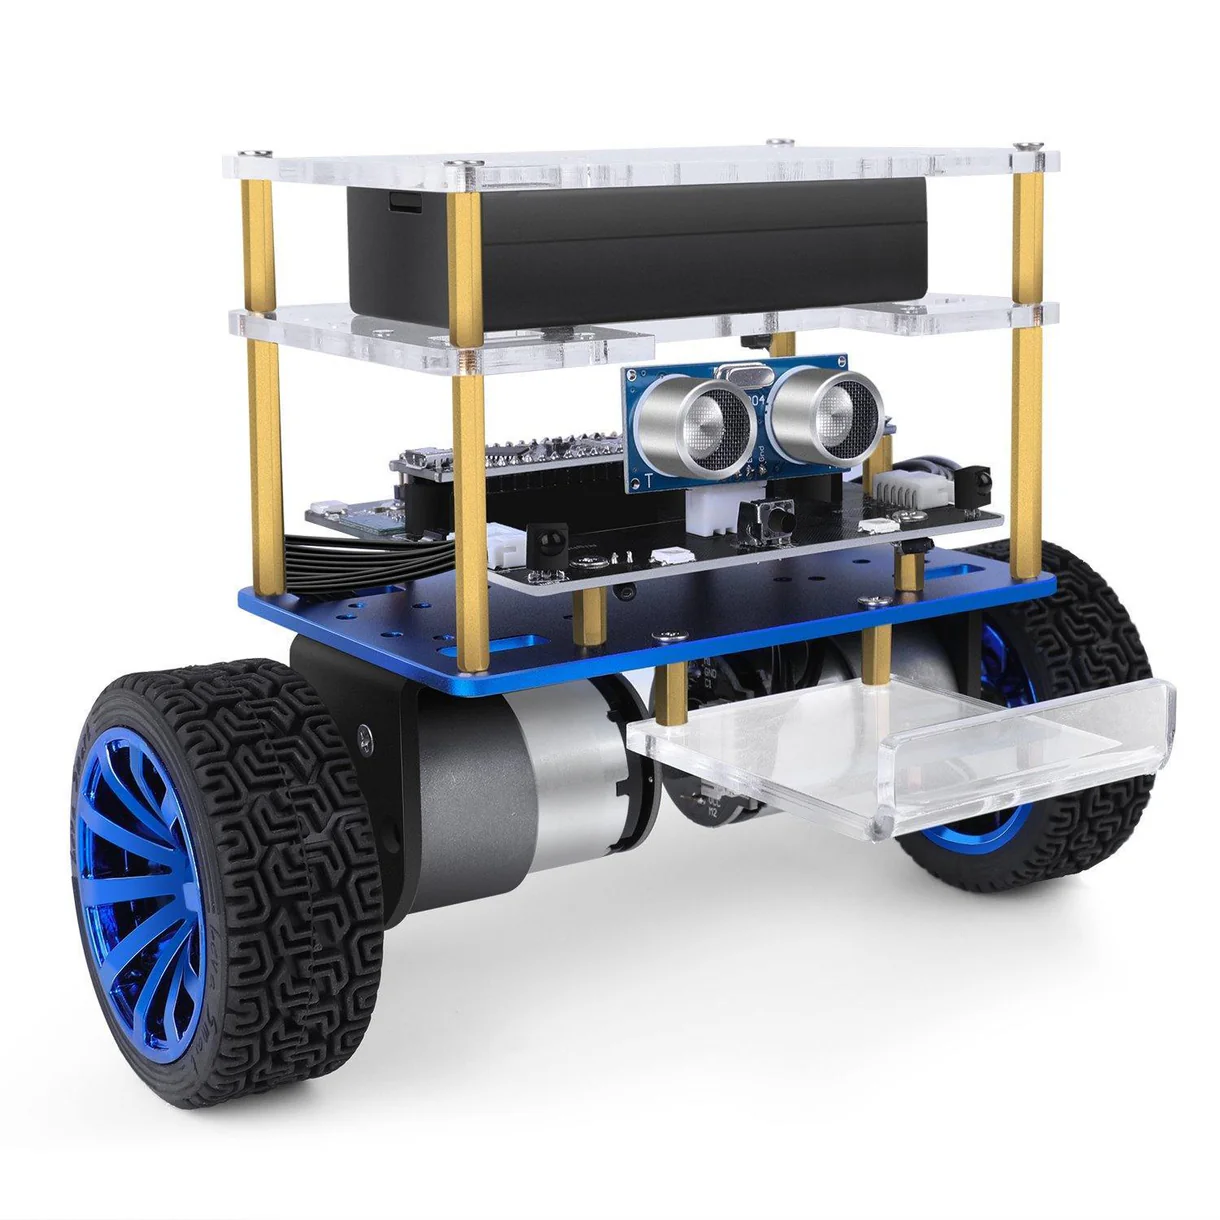
\includegraphics[width=0.7\textwidth, center]{img/elegoo_tumbller.png}
    \caption{Rendering des Elegoo Tumbller}
    \label{fig:elegoo_tumbller}
\end{figure}
\begin{sidewaysfigure}
    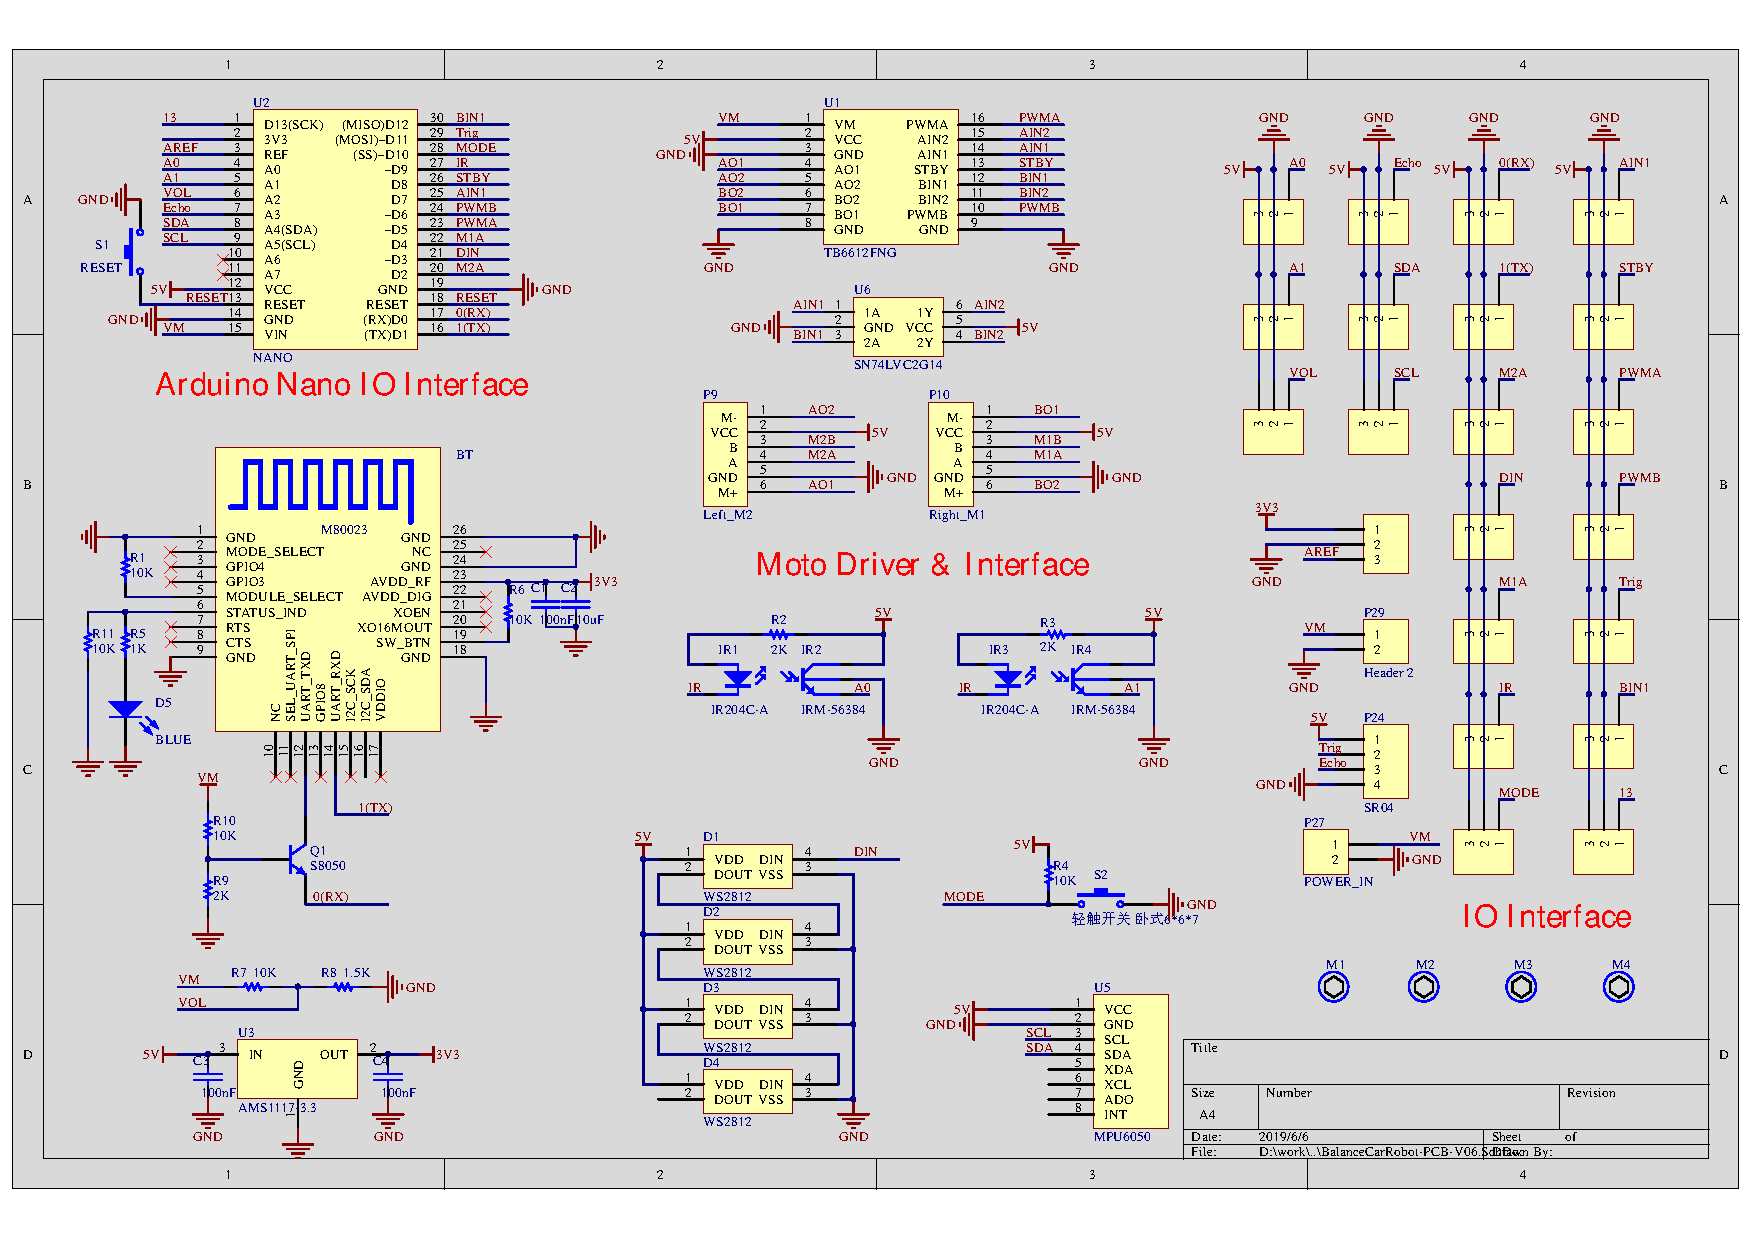
\includegraphics[width=\textwidth, center]{img/elegoo_tumbller_original_circuit.pdf}
    \caption{Originaler Schaltplan des Tumbllers (TODO: neu zeichnen)}
    \label{fig:elegoo_tumbller_original_circuit}
\end{sidewaysfigure}

\section{Guide}
\label{subsec:hardware_guide}
Die Aufgabe von \textit{Guide} ist es,
mithilfe eines LiDAR-Sensors (Siehe Kapitel \ref{subsec:ueberblick_lidar}) die Umgebung nach Hindernissen
und den anderen Robotern abzusuchen.
%
Die vom LiDAR gesammelten Abstandsdaten werden über eine TCP/IP Websocket-Verbindung
an einen zentralen Server weitergegeben,
welcher diese weiter verarbeitet.
%
Um den LiDAR-Sensor zu montieren,
haben wir das Fahrgestell leicht modifiziert
und die oberste Ebene (mit dem Akku) erhöht,
um Platz für Schrauben zu schaffen.

\section{Tamerlan \& Bambi}
\label{subsec:hardware_tamerlan_bambi}